\documentclass[letterpaper,11pt]{article}
\usepackage{latexsym}
\usepackage[empty]{fullpage}
\usepackage[usenames,dvipsnames]{color}
\usepackage{verbatim}
\usepackage{hyperref}
\usepackage{framed}
\usepackage{tocloft}
\usepackage{bibentry}
\usepackage{amsmath}
\usepackage{scrextend}
\usepackage{listings}
\usepackage{color}
\usepackage{fancyhdr}
\usepackage{graphicx}

%THIS PORTION IS FOR ADDING PAGE NUMBER
\pagestyle{fancy}
\cfoot{}
\rfoot{\thepage}
\renewcommand{\headrulewidth}{0pt}

%THIS PORTION IS FOR ADDING PAGE NUMBER
\urlstyle{same}
\definecolor{mygrey}{gray}{.85}
\definecolor{mygreylink}{gray}{.30}
\textheight=9.0in
\raggedbottom
\raggedright
\setlength{\tabcolsep}{0in}

%The following part is for inserting codes in LaTeX:
\definecolor{codegreen}{rgb}{0,0.6,0}
\definecolor{codegray}{rgb}{0.5,0.5,0.5}
\definecolor{codepurple}{rgb}{0.58,0,0.82}
\definecolor{backcolour}{rgb}{0.95,0.95,0.92}

\lstdefinestyle{mystyle}{
    backgroundcolor=\color{backcolour},
    commentstyle=\color{codegreen},
    keywordstyle=\color{magenta},
    numberstyle=\tiny\color{codegray},
    stringstyle=\color{codepurple},
    basicstyle=\footnotesize,
    breakatwhitespace=false,
    breaklines=true,
    captionpos=b,
    keepspaces=true,
    numbers=left,
    numbersep=5pt,
    showspaces=false,
    showstringspaces=false,
    showtabs=false,
    tabsize=2}
\lstset{style=mystyle}

% Adjust margins
\usepackage[left=0.9in,top=0.7in,right=0.9in,bottom=0.9in]{geometry}

%%%%%%%%%%%%%%%%%%%%%%%%%%%%%%%%%%%%%
%%%%%%   settings end here   %%%%%%%%
%%%%%%%%%%%%%%%%%%%%%%%%%%%%%%%%%%%%%

\begin{document}

\begin{center}
	\textbf{\Huge{Advanced Data Analysis HW4}}
\end{center}

\begin{center}
	\textsl{Ao Liu, al3472}
\end{center}

\bigbreak
\bigbreak
\bigbreak


%%%%%%%%%%%%%%%%%%%%%%%%%%%%%%%%%%%%%
%%%%%%%%%%%%%%   1   %%%%%%%%%%%%%%%%
%%%%%%%%%%%%%%%%%%%%%%%%%%%%%%%%%%%%%

\begin{addmargin}[-2em]{0em}
  \large{\textbf{1. }}
\end{addmargin}
\textbf{A national insurance organization wanted to study the consumption patter on cigarettes in all 50 states and the District of Columbia. The variables chosen for the study are}\par

\begin{center}
\begin{tabular}{ p{2cm}p{12cm} }\\
Variable & Definition\\
\hline
Age & Median age of the a person living in a state\\
HS & Percentage of people over 25 years of age in a state who had completed high school\\
Income & Per capita personal income for a state in dollars\\
Black & Percentage of blacks living in a state\\
Female & Percentage of females living in a state\\
Price & Weighted average price (in cents) of a pack of cigarettes in a state\\
Sales & Number of packs of cigarettes sold in a state on a per capita basis\\
\end{tabular}
\end{center}

\begin{addmargin}[-1.1em]{0em}
  \textbf{(a)}\par
\end{addmargin}
\textbf{What would you expect the relationship between Sales and each of the explanatory variables to be? explain.}\par
\bigbreak
\begin{addmargin}[-0.5em]{0em}
  \textbf{Answer: }
\end{addmargin}

I expect there's a positive correlation between sales of cigarettes and Age, because the people with higher ages tend to smoke more cigarettes, the proportion of people smoking within young people is relatively small.\par
I expect there's a negative correlation between sales of cigarettes and HS, because people with higher education are more aware of the harm of smoking and are tend to somke less.\par
I expect there's a positive correlation between sales of cigarettes and Income, because with more money, people can afford more cigarettes.\par
I don't expect there's a correlation between sales of cigarettes and Black, because there's no supporting evidence that black people are mode likely to smoke more than others.\par
I expect there's a negative correlation between sales of cigarettes and Female, because there are a lot more men smoking than women, the higher the proportion of the women, the less the proportion of people smoking.\par
I expect there's a negative correlation between sales of cigarettes and Price, the less the price is, the more people can afford the cigarettes.\par


\begin{addmargin}[-1.1em]{0em}
  \textbf{(b)}\par
\end{addmargin}
\textbf{Compute the pairwise correlation coefficient matrix and construct the corresponding scatter plot matrix}\par
\bigbreak
\begin{addmargin}[-0.5em]{0em}
  \textbf{Answer: }
\end{addmargin}

\begin{lstlisting}
> data = read.table("DATACIGARETTE.txt", header = TRUE)
> mat.data <- data.matrix(data[,2:8])
> cor((mat.data))
\end{lstlisting}
so the pairwise correlation coefficient matrix is:
\begin{lstlisting}
         Age	      HS	      Income	    Black	     Female	    Price	    Sales
  Age	1.00000000	-0.09891626	0.25658098	-0.04033021	0.55303189	0.24775673	0.22655492
  HS	-0.09891626	1.00000000	0.53400534	-0.50171191	-0.41737794	0.05697473	0.06669476
  Income	0.25658098	0.53400534	1.00000000	0.01728756	-0.06882666	0.21455717	0.32606789
  Black	-0.04033021	-0.50171191	0.01728756	1.00000000	0.45089974	-0.14777619	0.18959037
  Female	0.55303189	-0.41737794	-0.06882666	0.45089974	1.00000000	0.02247351	0.14622124
  Price	0.24775673	0.05697473	0.21455717	-0.14777619	0.02247351	1.00000000	-0.30062263
  Sales	0.22655492	0.06669476	0.32606789	0.18959037	0.14622124	-0.30062263	1.00000000
\end{lstlisting}


\begin{lstlisting}
> pairs(data[,2:8])
\end{lstlisting}

The corresponding scatter plot is:
\begin{center} \makebox[\linewidth]{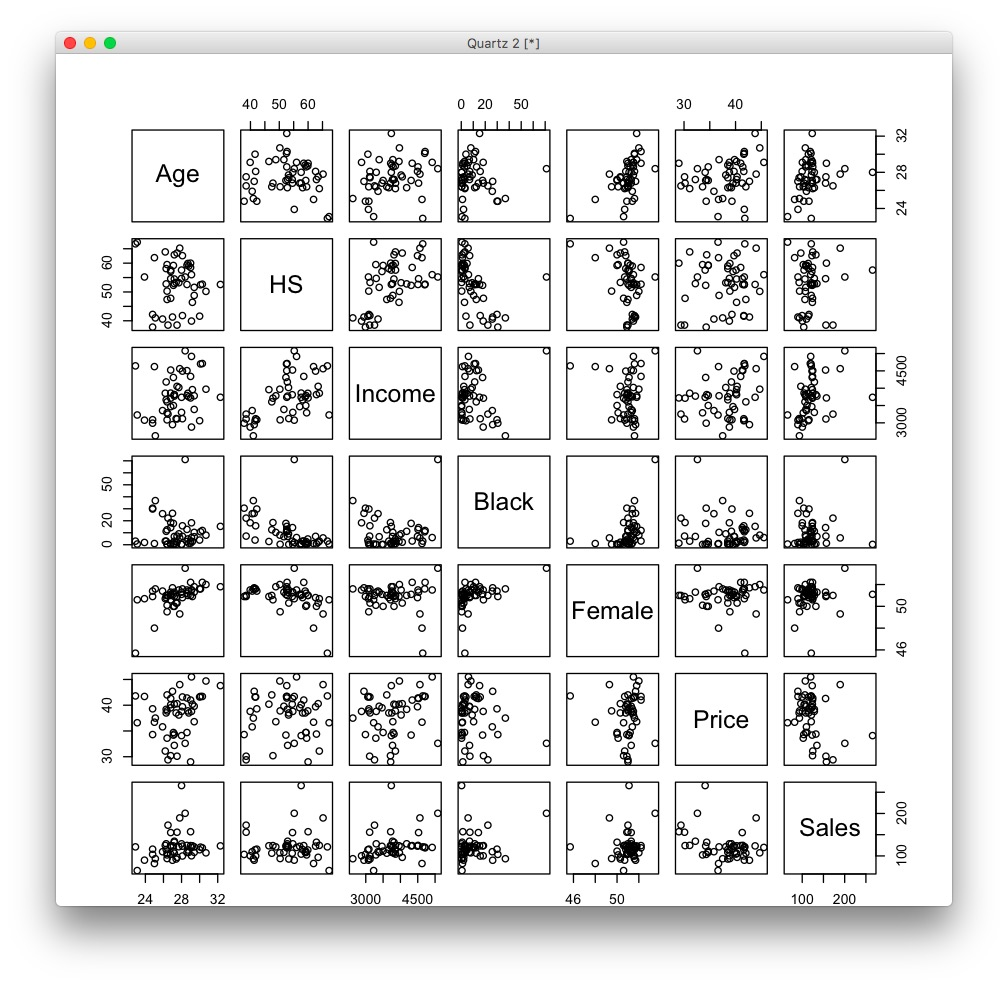
\includegraphics[width=\textwidth]{HW4.jpg}}
\end{center}

\begin{addmargin}[-1.1em]{0em}
  \textbf{(c)}\par
\end{addmargin}
\textbf{Obtain the six variance inflation factors. What do these results suggest about the effect of multicollinearity?}\par
\bigbreak
\begin{addmargin}[-0.5em]{0em}
  \textbf{Answer: }
\end{addmargin}

\begin{lstlisting}
> results = lm(Sales ~ Age+HS+Income+Black+Female+Price , data=data)
# install.packages('car')
> library(car)
> vif(results)
\end{lstlisting}
The VIF for 6 variables are:
\begin{lstlisting}
  Age       HS   Income    Black   Female    Price
2.300617 2.676465 2.325164 2.392152 2.406417 1.142181
\end{lstlisting}

\begin{addmargin}[-1.1em]{0em}
  \textbf{(d)}\par
\end{addmargin}
\textbf{Are the there any outlying Sales observations in the regres- sion model relating Sales to the six predictors?}\par
\bigbreak
\begin{addmargin}[-0.5em]{0em}
  \textbf{Answer: }
\end{addmargin}

Yes, there are outlying Sales observations in the regression model relating Sales to the six predictors.\par
\begin{lstlisting}
> r = rstudent(results)
> data[abs(r)>3,]
\end{lstlisting}

\begin{lstlisting}
  State	Age	HS	Income	Black	Female	Price	Sales
29	NV	27.8	65.2	4563	5.7	49.3	44.0	189.5
30	NH	28.0	57.6	3737	0.3	51.1	34.1	265.7
\end{lstlisting}

As we can see from the result, NV and NH are the two states that have outlying Sales observations in the regression model relating Sales to the six predictors.

\begin{addmargin}[-1.1em]{0em}
  \textbf{(e)}\par
\end{addmargin}
\textbf{Obtain the leverages (the diagonal elements of the hat matrix). Are the there any outlying states in the six predictors?}\par
\bigbreak
\begin{addmargin}[-0.5em]{0em}
  \textbf{Answer: }
\end{addmargin}

\begin{lstlisting}
> results = lm(Sales ~ Age+HS+Income+Black+Female+Price , data=data)
> lev = hat(model.matrix(results))
> lev
\end{lstlisting}

\begin{lstlisting}
  0.148834504030601 0.580160351053579 0.0496985364502016 0.13709423363853 0.0601062187168606 0.130138939805311 0.174671432351856 0.109964259157845 0.719712840922186 0.2984807799694 0.0992462576906176 0.216903455841289 0.092060813754798 0.078138923121058 0.0863031077553889 0.0600834204236368 0.0600531614367214 0.229271714316211 0.147216983914844 0.0592277100717082 0.082438148474407 0.111768500306865 0.0788600537461464 0.0595424855799236 0.220268293959589 0.0538126742130819 0.07535749988127 0.0713061951148198 0.171156408722539 0.0663450574293963 0.112543589203342 0.205163482615724 0.125210794051503 0.189612219012305 0.0977942068782977 0.0427023659576899 0.0747312407280888 0.194824611487451 0.110848283936785 0.107728709447137 0.157387827636549 0.0702636797470909 0.0861059621640753 0.073209300335295 0.310573704010913 0.0646432821046025 0.121378178796484 0.06441386857486 0.139413729014416 0.0386706972156815 0.0845573052310269
\end{lstlisting}

According to the common rule we will flag any observation whose leverage value satisfies
$$h_{ii} > \frac{2p}{n} = \frac{12}{51}$$

\begin{lstlisting}
> data[which(lev>12/51),1]
> lev[lev>12/51]
\end{lstlisting}

\begin{lstlisting}
AK DC FL UT
0.580160351053579 0.719712840922186 0.2984807799694 0.310573704010913
\end{lstlisting}

Thus, according to the rule above, we get 4 states who have high leverage: AK, DC, FL, UT.

\begin{addmargin}[-1.1em]{0em}
  \textbf{(f)}\par
\end{addmargin}
\textbf{Are there any influential points?}\par
\bigbreak
\begin{addmargin}[-0.5em]{0em}
  \textbf{Answer: }
\end{addmargin}

Typically, points with Cook's distance greater than 1 are classified as being influential, so we calculate Cook's distance for every state's data:
\begin{lstlisting}
> cook = cooks.distance(results)
> cook
\end{lstlisting}
Then we get the 51 Cook's distance:
\begin{lstlisting}
0.000872312260768373 0.11046568368098 0.000231406438616766 0.00533644985289951 0.00087184813943891 0.00487422897991362 0.000903689085754166 0.0247623942663158 0.272772360871267 0.00031718427842994 0.00228486844474409 0.149108047215374 0.00577305260600313 0.000515725336002152 0.000235292422912618 0.0022195814166927 0.0011742764662855 0.0293108038740074 0.0091907941594545 0.0046197884422297 0.00853949173434342 5.43666855436729e-05 0.000993543307494363 0.000416583654710988 0.00357717450931961 0.00181158830548335 0.00222167629931825 0.0106704252779454 0.226884733564416 0.243073931655456 0.00865807771956428 0.00862556323250348 0.0128750489379433 0.0514726373485391 0.000694147592466878 0.000198786969647856 0.000926126973805015 0.000632210801320141 0.00231792501997608 3.5406858359337e-07 0.00559710600247828 0.0021868920733631 0.000167678660476866 0.000276633855805063 0.0861896935150744 0.00441253690931487 0.0144781318896138 0.00554156138259945 0.00241683043673791 0.000216940322227759 6.00182901861485e-05
\end{lstlisting}
No one is greater than 1, so there's no influential points according to the rule of Cook's distance.

\begin{addmargin}[-1.1em]{0em}
  \textbf{(g)}\par
\end{addmargin}
\textbf{Use log(Sales) instead of Sales and repeat questions d), e) and f).}\par
\bigbreak
\begin{addmargin}[-0.5em]{0em}
  \textbf{Answer: }
\end{addmargin}

\begin{lstlisting}
> results = lm(log(Sales) ~ Age+HS+Income+Black+Female+Price, data=data)
> r = rstudent(results)
> data[abs(r)>3,]
\end{lstlisting}

\begin{lstlisting}
  State	Age	HS	Income	Black	Female	Price	Sales
29	NV	27.8	65.2	4563	5.7	49.3	44.0	189.5
30	NH	28.0	57.6	3737	0.3	51.1	34.1	265.7
\end{lstlisting}

As we can see from the result, NV and NH are the two states that have outlying Sales observations in the regression model relating Sales to the six predictors.

\begin{lstlisting}
> lev = hat(model.matrix(results))
> lev
\end{lstlisting}

\begin{lstlisting}
  0.148834504030601 0.580160351053579 0.0496985364502016 0.13709423363853 0.0601062187168606 0.130138939805311 0.174671432351856 0.109964259157845 0.719712840922186 0.2984807799694 0.0992462576906176 0.216903455841289 0.092060813754798 0.078138923121058 0.0863031077553889 0.0600834204236368 0.0600531614367214 0.229271714316211 0.147216983914844 0.0592277100717082 0.082438148474407 0.111768500306865 0.0788600537461464 0.0595424855799236 0.220268293959589 0.0538126742130819 0.07535749988127 0.0713061951148198 0.171156408722539 0.0663450574293963 0.112543589203342 0.205163482615724 0.125210794051503 0.189612219012305 0.0977942068782977 0.0427023659576899 0.0747312407280888 0.194824611487451 0.110848283936785 0.107728709447137 0.157387827636549 0.0702636797470909 0.0861059621640753 0.073209300335295 0.310573704010913 0.0646432821046025 0.121378178796484 0.06441386857486 0.139413729014416 0.0386706972156815 0.0845573052310269
\end{lstlisting}

According to the common rule we will flag any observation whose leverage value satisfies
$$h_{ii} > \frac{2p}{n} = \frac{12}{51}$$

\begin{lstlisting}
> data[which(lev>12/51),1]
> lev[lev>12/51]
\end{lstlisting}

\begin{lstlisting}
AK DC FL UT
0.580160351053579 0.719712840922186 0.2984807799694 0.310573704010913
\end{lstlisting}

Thus, according to the rule above, we get 4 states who have high leverage: AK, DC, FL, UT.

Typically, points with Cook's distance greater than 1 are classified as being influential, so we calculate Cook's distance for every state's data:
\begin{lstlisting}
> cook = cooks.distance(results)
> cook
\end{lstlisting}
Then we get the 51 Cook's distance:
\begin{lstlisting}
0.00359045513224516 0.240240855616072 0.00121318532616218 0.00940000348486041 0.000293993996183841 0.000845445364141786 0.00157627217231795 0.0336654337125128 0.14134926250704 4.17359595508581e-08 0.00203727701223271 0.270758042867878 0.00458499785548776 0.000451889520957869 9.31888737750166e-06 0.00184184619189831 0.000560973161470141 0.0319246707978281 0.0204097590400288 0.00921415105332014 0.00810736995024783 7.12278615229615e-05 0.00254520116778151 0.0002981214100366 0.00317957208142376 0.00184483532854467 0.00116873114507587 0.0108404640748746 0.242062092944229 0.161220045757967 0.0123781360184546 0.0103388197355609 0.0176912765990876 0.0540788613509783 0.00205060932036119 4.12952664005199e-05 0.000879330434682632 0.0030802159952135 0.00441873438600284 8.57636871488496e-05 0.005679380081201 0.00398597075671328 0.000654080555535082 0.00040384707347726 0.238154414273449 0.00956732233083818 0.0132426216290245 0.00700748304948474 0.00221365370129141 0.000195642965139178 0.00154531793916012
\end{lstlisting}
No one is greater than 1, so there's no influential points according to the rule of Cook's distance.

%%%%%%%%%%%%%%%%%%%%%%%%%%%%%%%%%%%%%
%%%%%%%%%%%%%%   2   %%%%%%%%%%%%%%%%
%%%%%%%%%%%%%%%%%%%%%%%%%%%%%%%%%%%%%

\begin{addmargin}[-2em]{0em}
  \large{\textbf{2. }}
\end{addmargin}
\textbf{Suppose that North American Oil Company is attempting to develop a regular gasoline that will deliver improved gasoline mileage. As part of its development process, the company would like to study the effect of two qualitative factors on the gasoline mileage obtained by an automobile called the Fire-Hawk. These factors are regular gasoline type (which has levels A, B and C) and gasoline additive type (which has levels M, N, O and P). To carry out the study, the company test drove three Fire-Hawks using each treatment. However upon completion of the experiment the company found that several Fire-Hawks have not been driven under the proper test conditions. Rather than running more tests, the company decided (because of limited time) to analyze the data that had remained after the data for improperly tested Fire-Hawks was dropped from the data set. The remaining data are in Oildata.cvs. Let}

$$yij,k = \textrm{the}\:k\textrm{th gasoline mileage obtained when using regular gasoline type}\: i \:\textrm{and additive type}\: j}$$

\textbf{A reasonable model to use for this data is}\par

$$y_{ijk} = \mu + \alpha_BD_{i,B} + \alpha_CD_{i,C} + \beta_ND_{j,N} + \beta_OD_{j,O} + \beta_PD_{j,P} + \epsilon_{ij,k}$$

\textbf{where}

\begin{center}
$D_{i,B} = 1$ if $i = B$, that is, if we are using gasoline type B and 0 otherwise\par
$D_{i,C} = 1$ if $i = C$, that is, if we are using gasoline type C and 0 otherwise\par
$D_{i,N} = 1$ if $i = N$, that is, if we are using additive type N and 0 otherwise\par
$D_{i,O} = 1$ if $i = O$, that is, if we are using additive type O and 0 otherwise\par
$D_{i,P} = 1$ if $i = P$, that is, if we are using additive type P and 0 otherwise\par
\end{center}


\begin{addmargin}[-1.1em]{0em}
  \textbf{(a)}\par
\end{addmargin}
\textbf{To compare the effects of the regular gasoline type, we need to test $H_0: \alpha_B =\alpha_C =0$ versus $H_a$: at least one of $\alpha_B$ or $\alpha_C$ does not equal zero.
}\par
\bigbreak
\begin{addmargin}[-0.5em]{0em}
  \textbf{Answer: }
\end{addmargin}

In order to test the hypothesis, we have a full model:

$$y_{ijk} = \mu + \alpha_BD_{i,B} + \alpha_CD_{i,C} + \beta_ND_{j,N} + \beta_OD_{j,O} + \beta_PD_{j,P} + \epsilon_{ij,k}$$

and a reduced model:
$$y_{ijk} = \mu + \beta_ND_{j,N} + \beta_OD_{j,O} + \beta_PD_{j,P} + \epsilon_{ij,k}$$

We will reject the Null Hypothesis if the two models are different:
\begin{lstlisting}
> data = read.csv("Oildata.csv")
> colnames(data)
> full = lm(Mileage ~ factor(Rgasoline) + factor(GasolineAd), data = data)
> reduce1 = lm(Mileage ~ factor(GasolineAd), data = data)
> anova(reduce1, full)
\end{lstlisting}

\begin{lstlisting}
Res.Df	RSS	      Df	Sum of Sq	 F	        Pr(>F)
37	    3496.295	NA	NA	       NA	        NA
35	    3466.153	2	  30.14234	 0.1521834	0.859396
\end{lstlisting}

Since the p-value of the test is $0.859396 > \alpha = 0.05$, we cannot reject the Null Hypothesis that $\alpha_B = \alpha_C = 0$


\begin{addmargin}[-1.1em]{0em}
  \textbf{(b)}\par
\end{addmargin}
\textbf{To compare the effects of the gasoline additive type, we need to test $H_0 :\beta_N =\beta_O =\beta_P =0$ versus $H_a$: at least one of $\beta_N,\beta_O,\beta_P$ does not equal zero.}\par
\bigbreak
\begin{addmargin}[-0.5em]{0em}
  \textbf{Answer: }
\end{addmargin}

 In order to test the hypothesis, we have a full model:

 $$y_{ijk} = \mu + \alpha_BD_{i,B} + \alpha_CD_{i,C} + \beta_ND_{j,N} + \beta_OD_{j,O} + \beta_PD_{j,P} + \epsilon_{ij,k}$$

 and a reduced model:
 $$y_{ijk} = \mu + \alpha_BD_{i,B} + \alpha_CD_{i,C} + \epsilon_{ij,k}$$

 We will reject the Null Hypothesis if the two models are different:
\begin{lstlisting}
 > full = lm(Mileage ~ factor(Rgasoline) + factor(GasolineAd), data = data)
 > reduce2 = lm(Mileage ~ factor(Rgasoline), data = data)
 > anova(reduce2, full)
\end{lstlisting}

\begin{lstlisting}
Res.Df RSS	     Df	 Sum of Sq	F	         Pr(>F)
38	   3592.151	 NA	 NA	        NA	       NA
35	   3466.153	 3	 125.9986	  0.4240966	 0.736912
\end{lstlisting}

Since the p-value of the test is $0.736912 > \alpha = 0.05$, we cannot reject the Null Hypothesis that $\beta_N = \beta_O =\beta_P = 0$

\end{document}

%%%%%%%%%%%%%%%%%%%%%%%%%%%%%%%%%%%%%
%%%%%%%%%%%%%%   #   %%%%%%%%%%%%%%%%
%%%%%%%%%%%%%%%%%%%%%%%%%%%%%%%%%%%%%

%Insert pics:
%%%%%%%%%%%%%
%\begin{center}
  %\makebox[\linewidth]{\includegraphics[width=\textwidth]{4640HW6.jpg}}
%\end{center}

%insert a complicated tab...
%%%%%%%%%%%%%%%%%%%%%%%%%%%%
%\begin{center}
%\begin{tabular}{ p{12cm}p{1cm}p{1cm}p{1cm}  }
%& \multicolumn{3}{c}{Posterior Quantiles} \\
%\centering{Quantity of Interest} & 25\% & 50\% & 75\% \\
%\hline
%geometric mean for Blue Earth (no basement), exp($\beta_2)$ &4.1& 5.0& 6.5\\
%geometric mean for Blue Earth County (basement), exp($\beta_1+\beta_2)$ &6.1 &7.1 &8.2\\
%geometric mean for Clay County (no basement), exp($\beta_3)$& 3.8& 4.7 &5.8\\
%geometric mean for Clay County (basement), exp($\beta_1+\beta_3)$ &5.6& 6.5& 7.6\\
%geometric mean for Goodhue County (no basement), exp($\beta_4)$ & 3.9 &4.9& 6.2\\
%geometric mean for Goodhue County (basement), exp($\beta_1+\beta_4)$ &5.8& 6.8& 7.9\\
%factor for basement vs. no basement, exp($\beta_1$)&1.1& 1.4 &1.7\\
%geometric sd of predictions, exp($\sigma$)&2.1 &2.2& 2.4\\
%\end{tabular}
%\end{center}

%%%insert code snippets:
%%%%%%%%%%%%%%%%%%%%%%%%
%\begin{lstlisting}
%INSERT CODE HERE
%\end{lstlisting}

%%insert equation with severl lines:
%\begin{align}
%LEFT &= RIGHT1 \nonumber\\
%     &= RIGHT2 \nonumber\\
%     &= RIGHT3 \nonumber
%\end{align}


%ssh-add ~/.ssh/id_rsa
